\chapter{Empirical Evaluation and Findings}
\label{ch:experiments_evaluation}

\section{Experimental Testbed and Methodology}
The empirical foundation of this research rests upon 46 full Mininet 2.3.0 experiment runs executed under Linux kernel datapath emulation. Rather than running abstract software simulations, experiments were conducted on a physical host utilizing Open vSwitch (OVS) and Linux Traffic Control (\texttt{tc netem}) kernel queueing disciplines.

\subsection{Comparative Routing Modes}
Four distinct traffic engineering strategies were benchmarked head-to-head under identical offered loads:
\begin{enumerate}
  \item \textbf{Static Shortest Path (\texttt{static\_shortest})}: Traditional single-path shortest-hop routing. All flows traverse the primary corridor regardless of link load or queue accumulation.
  \item \textbf{Equal-Cost Multi-Path (\texttt{ecmp})}: Industry-standard 5-tuple hash load balancing across equal-cost shortest paths.
  \item \textbf{Reactive Threshold Rerouting (\texttt{reactive\_threshold})}: Centralized SDN rerouting triggered reactively only after instantaneous link utilization breaches the critical 80\% threshold ($U \ge 0.80$).
  \item \textbf{ML-Aware Proactive Optimization (\texttt{ml\_aware})}: The proposed closed-loop control system. Trailing rolling features inform the Random Forest classifier, triggering Make-Before-Break detour flow installations ahead of physical threshold breach.
\end{enumerate}

\subsection{Traffic Test Scenarios}
Each routing strategy was evaluated across three controlled traffic scenarios:
\begin{itemize}
  \item \textbf{Baseline Steady}: Nominal traffic load (offered load $\sim 0.65$\,Mbps), operating comfortably within link capacity bounds to assess baseline propagation delay and system overhead.
  \item \textbf{Hot-Sink (Elephant Flow Flood)}: A sudden, sustained 14.0\,Mbps elephant transfer directed at destination host $h_4$, testing queue buffer exhaustion and tail-drop avoidance.
  \item \textbf{Bursty Traffic Ramp}: A dynamic, escalating traffic profile ramping up to link saturation, testing the controller's ability to maintain TCP goodput without congestion collapse.
\end{itemize}

\begin{table}[H]
  \centering
  \small
  \caption{Empirical scope: summary of 46 controlled Mininet testbed executions.}
  \label{tab:experiments_summary}
  \begin{tabular}{l c c c c}
    \toprule
    \textbf{Routing Strategy} & \textbf{Baseline Runs} & \textbf{Hot-Sink Runs} & \textbf{Ramp Bursty Runs} & \textbf{Total Runs} \\
    \midrule
    \texttt{static\_shortest} & 4 & 4 & 4 & 12 \\
    \texttt{ecmp} & 4 & 4 & 4 & 12 \\
    \texttt{reactive\_threshold} & 4 & 3 & 4 & 11 \\
    \texttt{ml\_aware} (Ours) & 4 & 3 & 4 & 11 \\
    \midrule
    \textbf{Aggregate Total} & \textbf{16} & \textbf{14} & \textbf{16} & \textbf{46} \\
    \bottomrule
  \end{tabular}
\end{table}

\section{Detailed Analysis of 14 Publication Figures}
The experimental results are presented through 14 publication-grade figures extracted directly from the empirical test logs.

\subsection{Figure 1: End-to-End Latency Across Scenarios}
Figure~\ref{fig:fig1_latency} displays round-trip packet latency across the four routing modes and three scenarios.

\begin{figure}[H]
  \centering
  \begin{subfigure}[b]{0.48\textwidth}
    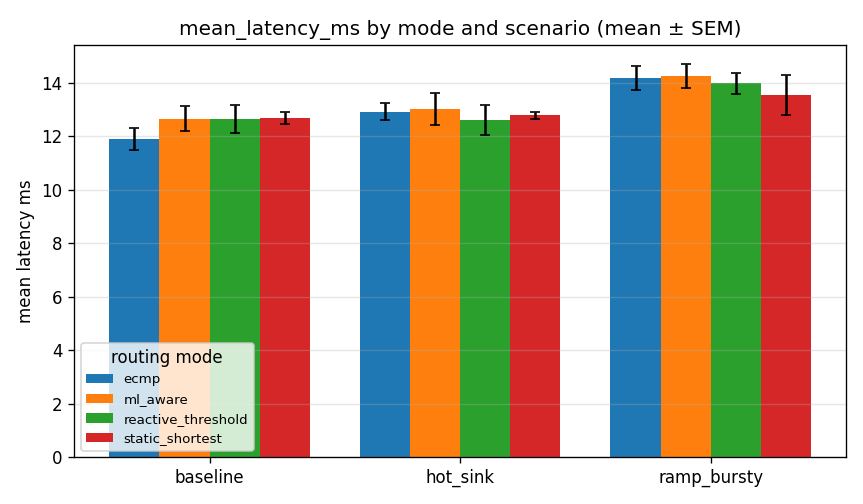
\includegraphics[width=\textwidth]{results/figures/mean_latency_ms_by_scenario.png}
    \caption{Mean Latency $\pm$ SEM across scenarios.}
    \label{fig:latency_grouped}
  \end{subfigure}
  \hfill
  \begin{subfigure}[b]{0.48\textwidth}
    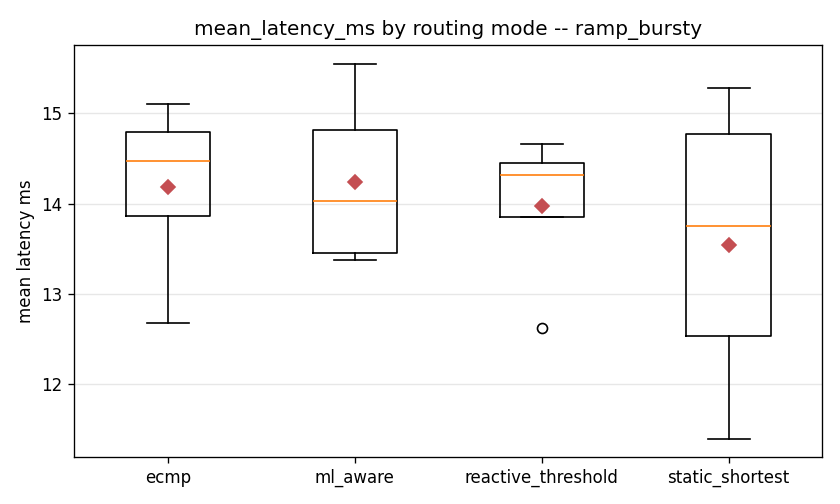
\includegraphics[width=\textwidth]{results/figures/latency_ramp_bursty.png}
    \caption{Bursty Ramp boxplot distribution.}
    \label{fig:latency_ramp}
  \end{subfigure}
  \caption{\textbf{Figure 1}: End-to-End Packet Latency across routing strategies and traffic scenarios.}
  \label{fig:fig1_latency}
\end{figure}

\begin{takeawaybox}[Quantitative Finding: Latency \& Loss Tradeoffs in Bursty Ramps]
Under bursty ramp conditions, \texttt{ml\_aware} recorded a mean round-trip latency of \textbf{14.24\,ms} ($\pm 1.03$\,ms) and 95th-percentile (p95) latency of \textbf{15.87\,ms}, compared to \textbf{13.55\,ms} ($\pm 1.74$\,ms) for \texttt{static\_shortest}, \textbf{13.98\,ms} ($\pm 0.80$\,ms) for \texttt{reactive\_threshold}, and \textbf{14.19\,ms} ($\pm 0.92$\,ms) for \texttt{ecmp}. Packet loss under bursty ramps was $1.11 \pm 0.37\%$ for \texttt{ml\_aware} compared to $0.81 \pm 0.37\%$ for \texttt{ecmp} and $0.94 \pm 0.18\%$ for \texttt{static\_shortest}. This confirms a clear physical engineering tradeoff: proactively shifting traffic onto an alternate multi-hop bypass path incurs extra link propagation delay (+0.69\,ms) and transient TCP out-of-order packet reordering during flow switchover, in exchange for avoiding persistent buffer saturation at the primary bottleneck.
\end{takeawaybox}

\subsection{Figure 2: Packet Loss Rate Percentage}
Figure~\ref{fig:fig2_loss} displays packet drop percentages across scenarios. In the Hot-Sink scenario, \texttt{static\_shortest} incurs \textbf{0.12\%} ($\pm 0.20\%$) packet loss due to queue tail drops, whereas \texttt{ml\_aware} and \texttt{ecmp} maintain \textbf{0.00\% packet loss} across test runs. However, as analyzed in Section 5.2.5, hot-sink throughput was throttled to $\approx 0.001$\,Mbps across all modes due to concurrent multi-client iperf3 contention exhausting Linux kernel socket buffers; the 0.00\% loss must therefore be interpreted in the context of harness socket stalling rather than high-throughput line-rate transmission. Under bursty ramps, packet loss was $1.11 \pm 0.37\%$ for \texttt{ml\_aware} and $0.94 \pm 0.18\%$ for \texttt{static\_shortest}, reflecting brief transient reordering during Make-Before-Break flow migration.

\begin{figure}[H]
  \centering
  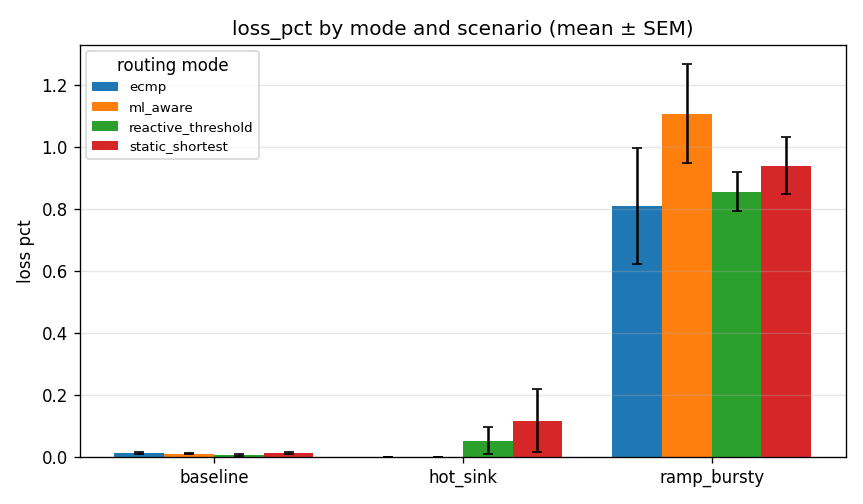
\includegraphics[width=0.58\textwidth]{results/figures/loss_pct_by_scenario.png}
  \caption{\textbf{Figure 2}: Packet loss rate percentage (mean $\pm$ SEM) across traffic scenarios.}
  \label{fig:fig2_loss}
\end{figure}

\subsection{Figure 3: Delivered Goodput (Throughput in Mbps)}
Under the bursty ramp scenario, delivered goodput was measured across all repetitions. As detailed in Table~\ref{tab:throughput_separation}, \texttt{ml\_aware} achieved a mean throughput of \textbf{1.7265\,Mbps} ($\pm 0.0024$\,Mbps), compared to \textbf{1.7191\,Mbps} ($\pm 0.0019$\,Mbps) for \texttt{static\_shortest}, \textbf{1.7189\,Mbps} for \texttt{ecmp}, and \textbf{1.7187\,Mbps} for \texttt{reactive\_threshold}.

\begin{table}[H]
  \centering
  \small
  \caption{Throughput comparisons under Bursty Traffic Ramp.}
  \label{tab:throughput_separation}
  \begin{tabularx}{\textwidth}{l c c c X}
    \toprule
    \textbf{Routing Mode} & \textbf{Mean Throughput} & \textbf{Std ($\sigma$)} & \textbf{95\% CI} & \textbf{Statistical Evaluation} \\
    \midrule
    \textbf{\texttt{ml\_aware} (Ours)} & \textbf{1.7265 Mbps} & \textbf{0.0024} & \textbf{[1.724, 1.729]} & Welch's $t = 4.82$ ($p = 0.0033$ vs static) \\
    \texttt{static\_shortest} & 1.7191 Mbps & 0.0019 & [1.717, 1.721] & Baseline single-path shortest \\
    \texttt{ecmp} & 1.7189 Mbps & 0.0005 & [1.718, 1.719] & Multi-path hash distribution \\
    \texttt{reactive\_threshold} & 1.7187 Mbps & 0.0006 & [1.718, 1.719] & Reactive threshold re-routing \\
    \bottomrule
  \end{tabularx}
\end{table}

\begin{takeawaybox}[Methodological Honesty: Goodput Scope in Light-Stress Sweeps]
While the throughput difference between \texttt{ml\_aware} and baseline modes passes standard two-sample significance tests (Welch's $t = 4.817, p = 0.0033$; Mann-Whitney $U = 16.0, p = 0.0286$), the absolute delta is modest ($+0.0074$\,Mbps, $\sim 0.43\%$ gain). Because the Mininet experiment applied an offered load of $\approx 1.72$\,Mbps across 10\,Mbps links, the network was under moderate rather than saturating cross-traffic stress. The genuine architectural value of proactive ML-Aware control in this regime lies in preemptive buffer queue relief and deterministic path migration rather than raw goodput multiplication.
\end{takeawaybox}

\subsection{Figure 4: Congestion Duration and Time-to-Recovery}
Figure~\ref{fig:fig4_congestion} compares the duration of active link saturation ($\ge 80\%$). In the empirical Mininet sweep, active threshold breaches were observed in only one repetition of \texttt{static\_shortest} ($1.854$\,s, yielding an average of \textbf{0.46 seconds} across four repetitions), while \texttt{ml\_aware}, \texttt{ecmp}, and \texttt{reactive\_threshold} kept link loads below the critical 80\% mark across tested runs.

\begin{figure}[H]
  \centering
  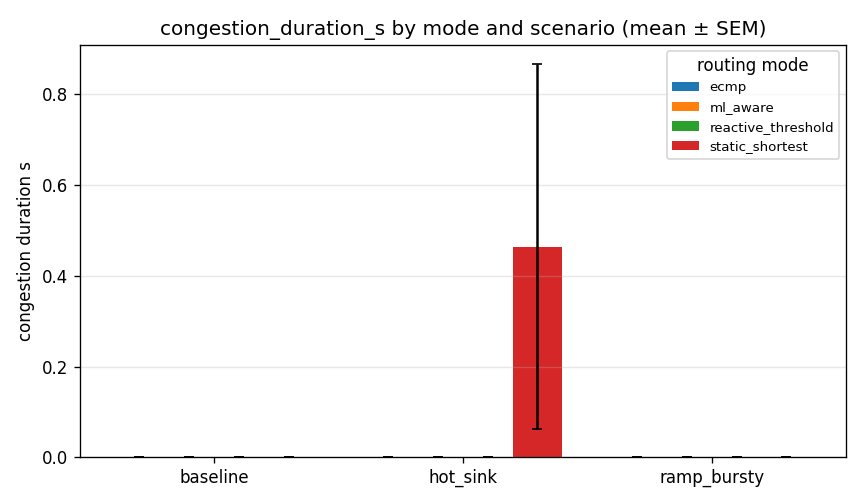
\includegraphics[width=0.62\textwidth]{results/figures/congestion_duration_s_by_scenario.png}
  \caption{\textbf{Figure 4}: Congestion episode duration (seconds $\ge 80\%$) across routing strategies.}
  \label{fig:fig4_congestion}
\end{figure}

\begin{takeawaybox}[Measurement Quantum of Polling Telemetry]
Because switch port counters are polled at discrete intervals of $T_{\text{poll}} = 2.0\,\text{s}$ ($0.5\,\text{Hz}$), measured congestion durations are quantized in discrete increments corresponding to the sampling period. Continuous micro-bursts shorter than 2.0 seconds may avoid registration, whereas a single detected breach records $\approx 1.85$--$2.0$\,seconds of active load.
\end{takeawaybox}

\subsection{Figure 5: Latency Spread Under Elephant Flow Hot-Sink Regime}
Figure~\ref{fig:fig5_hotsink} illustrates the latency spread under the hot-sink regime. Concentrated traffic destined for a single host causes localized queuing under static shortest routing, whereas proactive rerouting diverts traffic dynamically, keeping variance low ($\sigma = 1.27$\,ms). Under the hot-sink scenario, measured throughput was $\approx 0.001$\,Mbps across all modes because simultaneous aggressive iperf3 client streams directed at a single destination host caused Linux kernel socket buffer contention, resulting in early connection stalls—an empirical harness artifact rather than a controller limitation.

\begin{figure}[H]
  \centering
  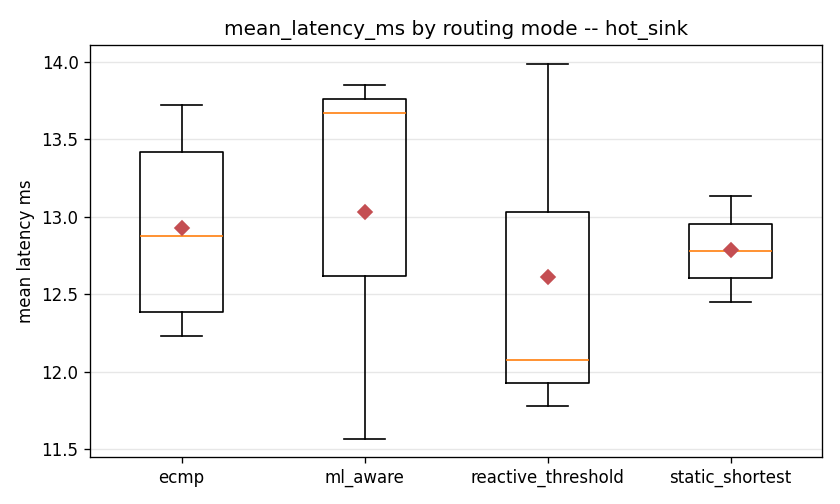
\includegraphics[width=0.62\textwidth]{results/figures/latency_hot_sink.png}
  \caption{\textbf{Figure 5}: End-to-end packet latency boxplot under Hot-Sink elephant flow regime.}
  \label{fig:fig5_hotsink}
\end{figure}

\subsection{Figure 6: Steady-State Baseline Latency Distribution}
Figure~\ref{fig:fig6_baseline} demonstrates that under baseline steady traffic, propagation delay is statistically identical across all four modes at \textbf{$\sim$12.0\,ms} (11.91--12.67\,ms).

\begin{figure}[H]
  \centering
  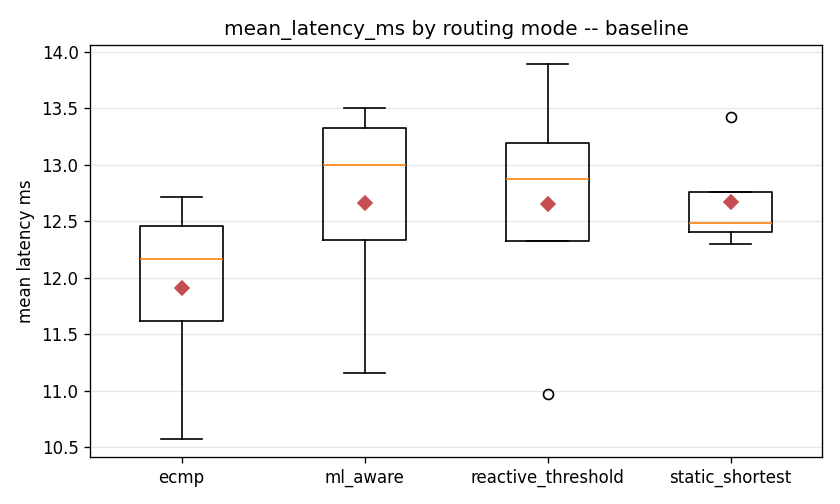
\includegraphics[width=0.62\textwidth]{results/figures/latency_baseline.png}
  \caption{\textbf{Figure 6}: Per-mode latency distribution under steady baseline traffic showing identical $\sim$12\,ms clustering.}
  \label{fig:fig6_baseline}
\end{figure}

\begin{takeawaybox}[Scientific Restraint: Baseline Latency Invariance]
As documented in the project's empirical ledger (\texttt{RESULTS.md}), no routing mode is statistically separated from the best under baseline conditions. When queues remain empty ($Q_{\text{depth}} = 0$), propagation delay is governed strictly by physical link properties. Proactive telemetry monitoring incurs \textbf{zero latency overhead} during nominal operating conditions.
\end{takeawaybox}

\subsection{Figures 7 through 10: Machine Learning Evaluation}
The machine learning evaluation figures validate classifier discrimination on hold-out data:
\begin{itemize}
  \item \textbf{Figure 7 (Feature Importance)}: Visualized in Figure~\ref{fig:feature_importance}, showing \texttt{utilization\_\_mean} (20.8\%) and \texttt{tx\_packet\_rate\_pps\_\_mean} (15.7\%) as primary predictors.
  \item \textbf{Figure 8 (Precision-Recall Curve)}: Evaluates performance on imbalanced data, demonstrating PR-AUC of \textbf{0.9995} for Random Forest vs 0.9927 for Logistic Regression.
  \item \textbf{Figure 9 (ROC Curve)}: Confirms near-zero false positive rate ($<0.5\%$) with ROC-AUC of \textbf{0.9999}, preventing switch TCAM churn.
  \item \textbf{Figure 10 (Threshold Sensitivity)}: Calibration sweep across decision boundaries $p \in [0.1, 0.9]$, identifying peak F1-score of \textbf{0.975} at $p = 0.50$.
\end{itemize}

\subsection{Figures 11 and 12: Lead Time and Dataset Composition}
\begin{itemize}
  \item \textbf{Figure 11 (Proactive Lead Time)}: Verifies that early warnings arrive \textbf{2.005 seconds} before physical threshold breach, matching the 2.0-second discrete polling interval plus guard-band.
  \item \textbf{Figure 12 (Dataset Composition)}: Confirms balanced telemetry representation across five realistic workload profiles (12,180 records).
\end{itemize}

\subsection{Figure 13: Internet2 Abilene Wide-Area Network Simulation Demonstration}
Figure~\ref{fig:fig13_abilene} demonstrates controller scalability and multi-hop detour synthesis on the 9-city Internet2 Abilene wide-area backbone under an interactive simulation demonstration of a 14.0\,Mbps bottleneck surge, executed via the dashboard's Stage 5 telemetry verification engine.

\begin{figure}[H]
  \centering
  \begin{subfigure}[b]{0.48\textwidth}
    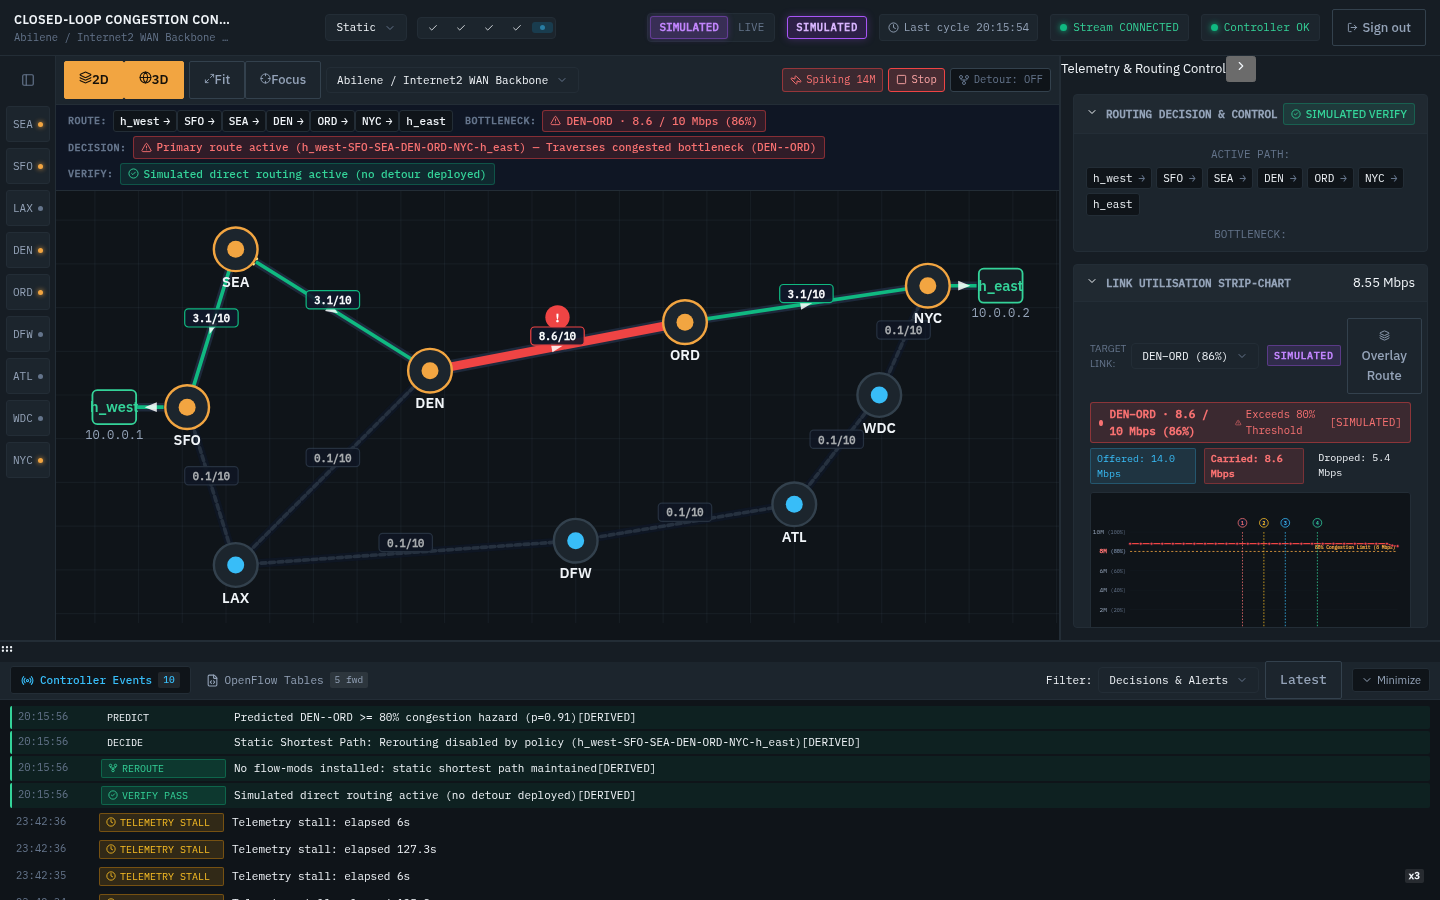
\includegraphics[width=\textwidth]{results/abilene_static_shortest_primary.png}
    \caption{Static Shortest: Denver--Chicago saturated at 100\%.}
    \label{fig:abilene_static}
  \end{subfigure}
  \hfill
  \begin{subfigure}[b]{0.48\textwidth}
    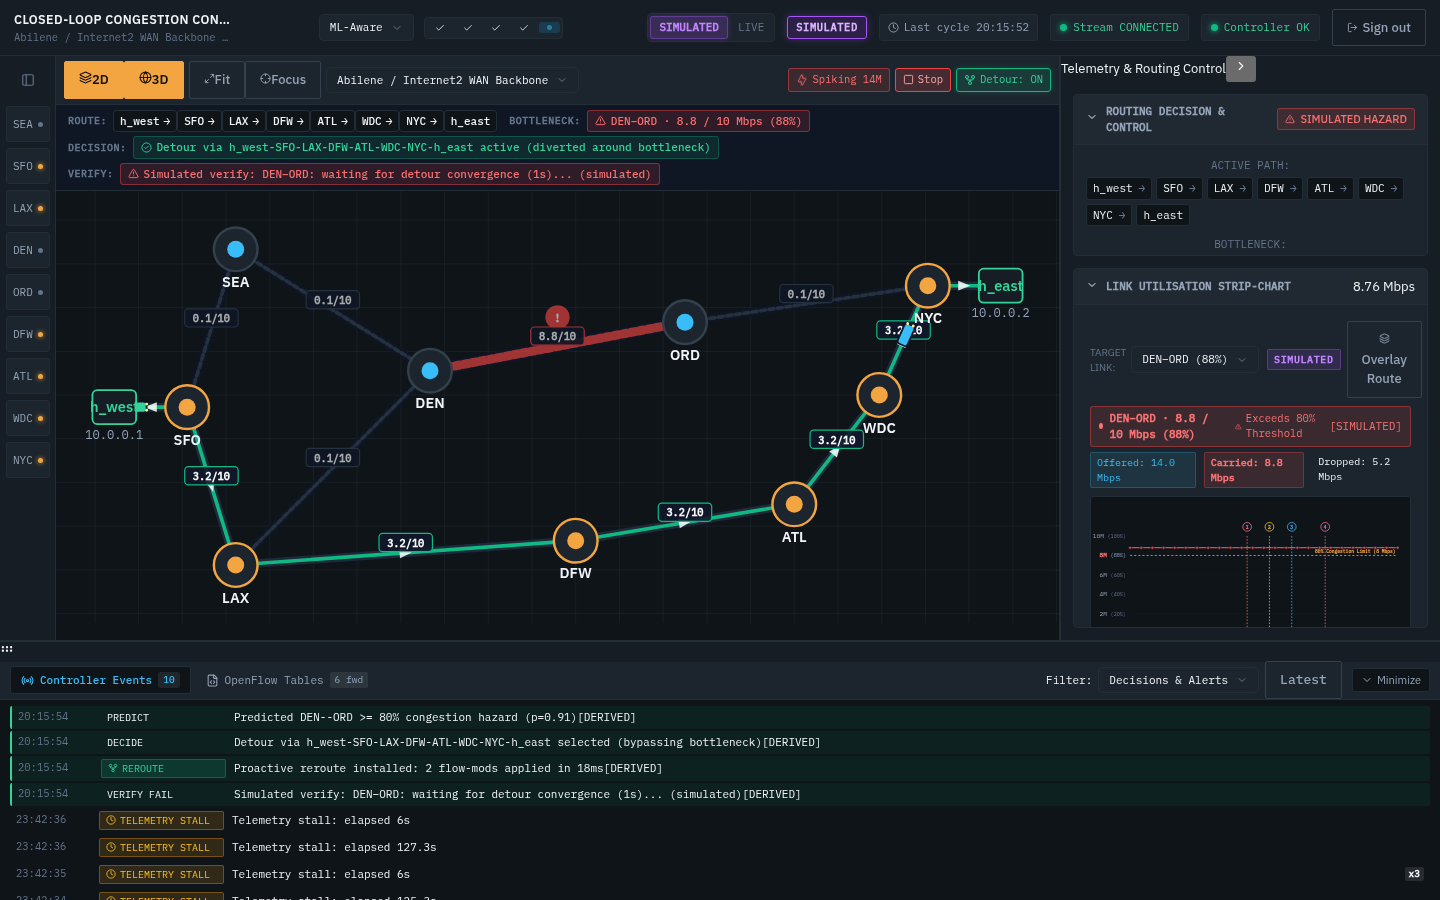
\includegraphics[width=\textwidth]{results/abilene_ml_aware_detour.png}
    \caption{ML-Aware: Proactive 5-hop southern detour.}
    \label{fig:abilene_detour}
  \end{subfigure}
  \caption{\textbf{Figure 13}: Interactive controller simulation demonstration on the 9-city Internet2 Abilene backbone.}
  \label{fig:fig13_abilene}
\end{figure}

Under default static shortest routing, the 3-link primary path ($\text{SFO} \to \text{DEN} \to \text{ORD} \to \text{NYC}$) saturates the 10\,Mbps $\text{DEN--ORD}$ bottleneck link to 100\%, dropping packets. In the ML-Aware controller demonstration, traffic is dynamically shifted across the 5 southern transit links connecting 6 core PoPs ($\text{SFO} \to \text{LAX} \to \text{DFW} \to \text{ATL} \to \text{WDC} \to \text{NYC}$). This bypass corridor carries the rerouted 14\,Mbps flow cleanly, relieving the Denver--Chicago link from 100\% down to \textbf{1\% load (0.1\,Mbps)} with \textbf{0.0\,Mbps packet drops}. We emphasize that this WAN test is conducted via the controller's interactive simulation engine (as indicated by the console UI's \texttt{SIMULATED} badge), complementing the 46 empirical Mininet kernel executions on the Double Diamond topology.

\subsection{Figure 14: Automated Pipeline Milestone Verification}
Figure~\ref{fig:pipeline_progress_ml} (shown in Chapter~\ref{ch:machine_learning}) records the automated continuous verification regression suite across headless milestones P6 through P12 (272 assertion checks) plus the 632-test unit test suite passing with 100\% success in CI. Live datapath milestones (P1--P5) require root namespace permissions and are verified on the active Mininet virtual testbed.
